
\begin{frame}{Spinner vs ListView en Android}
\textbf{¿Qué es un Spinner?}

\begin{itemize}
    \item Es un componente que permite seleccionar una opción de una lista desplegable.
    \item Ocupa poco espacio en pantalla.
    \item Ideal cuando se requiere elegir una sola opción entre varias.
\end{itemize}

\vspace{0.4cm}

\textbf{¿Qué es un ListView?}

\begin{itemize}
    \item Es un componente que muestra una lista de elementos visibles en pantalla.
    \item Permite visualizar múltiples opciones al mismo tiempo.
    \item Puede soportar selección simple o múltiple.
\end{itemize}

\vspace{0.4cm}

\textbf{Diferencias principales:}

\begin{itemize}
    \item \textbf{Espacio:} Spinner es compacto, ListView requiere más espacio.
    \item \textbf{Interacción:} Spinner usa menú desplegable, ListView muestra lista directa.
    \item \textbf{Uso:} Spinner para selección rápida; ListView para exploración de datos.
    \item \textbf{Cantidad de datos:} ListView es más adecuado para listas largas.
\end{itemize}

\end{frame}



\begin{frame}[fragile]
\frametitle{Demo 07: Agregar un Spinner}
\begin{columns}
\column{0.80\linewidth}
Del Repositorio Github:
\begin{itemize}
\item Copiar el archivo MainActivity\_Demo07.java (dentro del Folder códigosJAVA) al mismo directorio donde esta el MainActivity.java
\item Copiar el archivo activity\_main\_demo07.xml (dentro del Folder Carpeta\_layout) al mismo directorio donde esta el activity\_main.xml
%\item Copiar los archivos \textit{cgup.jpg} y \textit{logo\_upv\_2019.png} localizados dentro de la folder \textit{Carpeta\_drawable} en el directorio \textit{res/drawable} del proyecto de AS.
\item Modificar en el archivo AndroidManifest.xml la cadena \textit{.MainActivity\_Demo06} por \textit{.MainActivity\_Demo07}
\end{itemize}

\begin{block}{Demo \#07}
Muestra una App con un ListView. El usuario agregar elementos al presionar el boton superior.    
\end{block}


\column{0.20\linewidth}

\begin{center}
 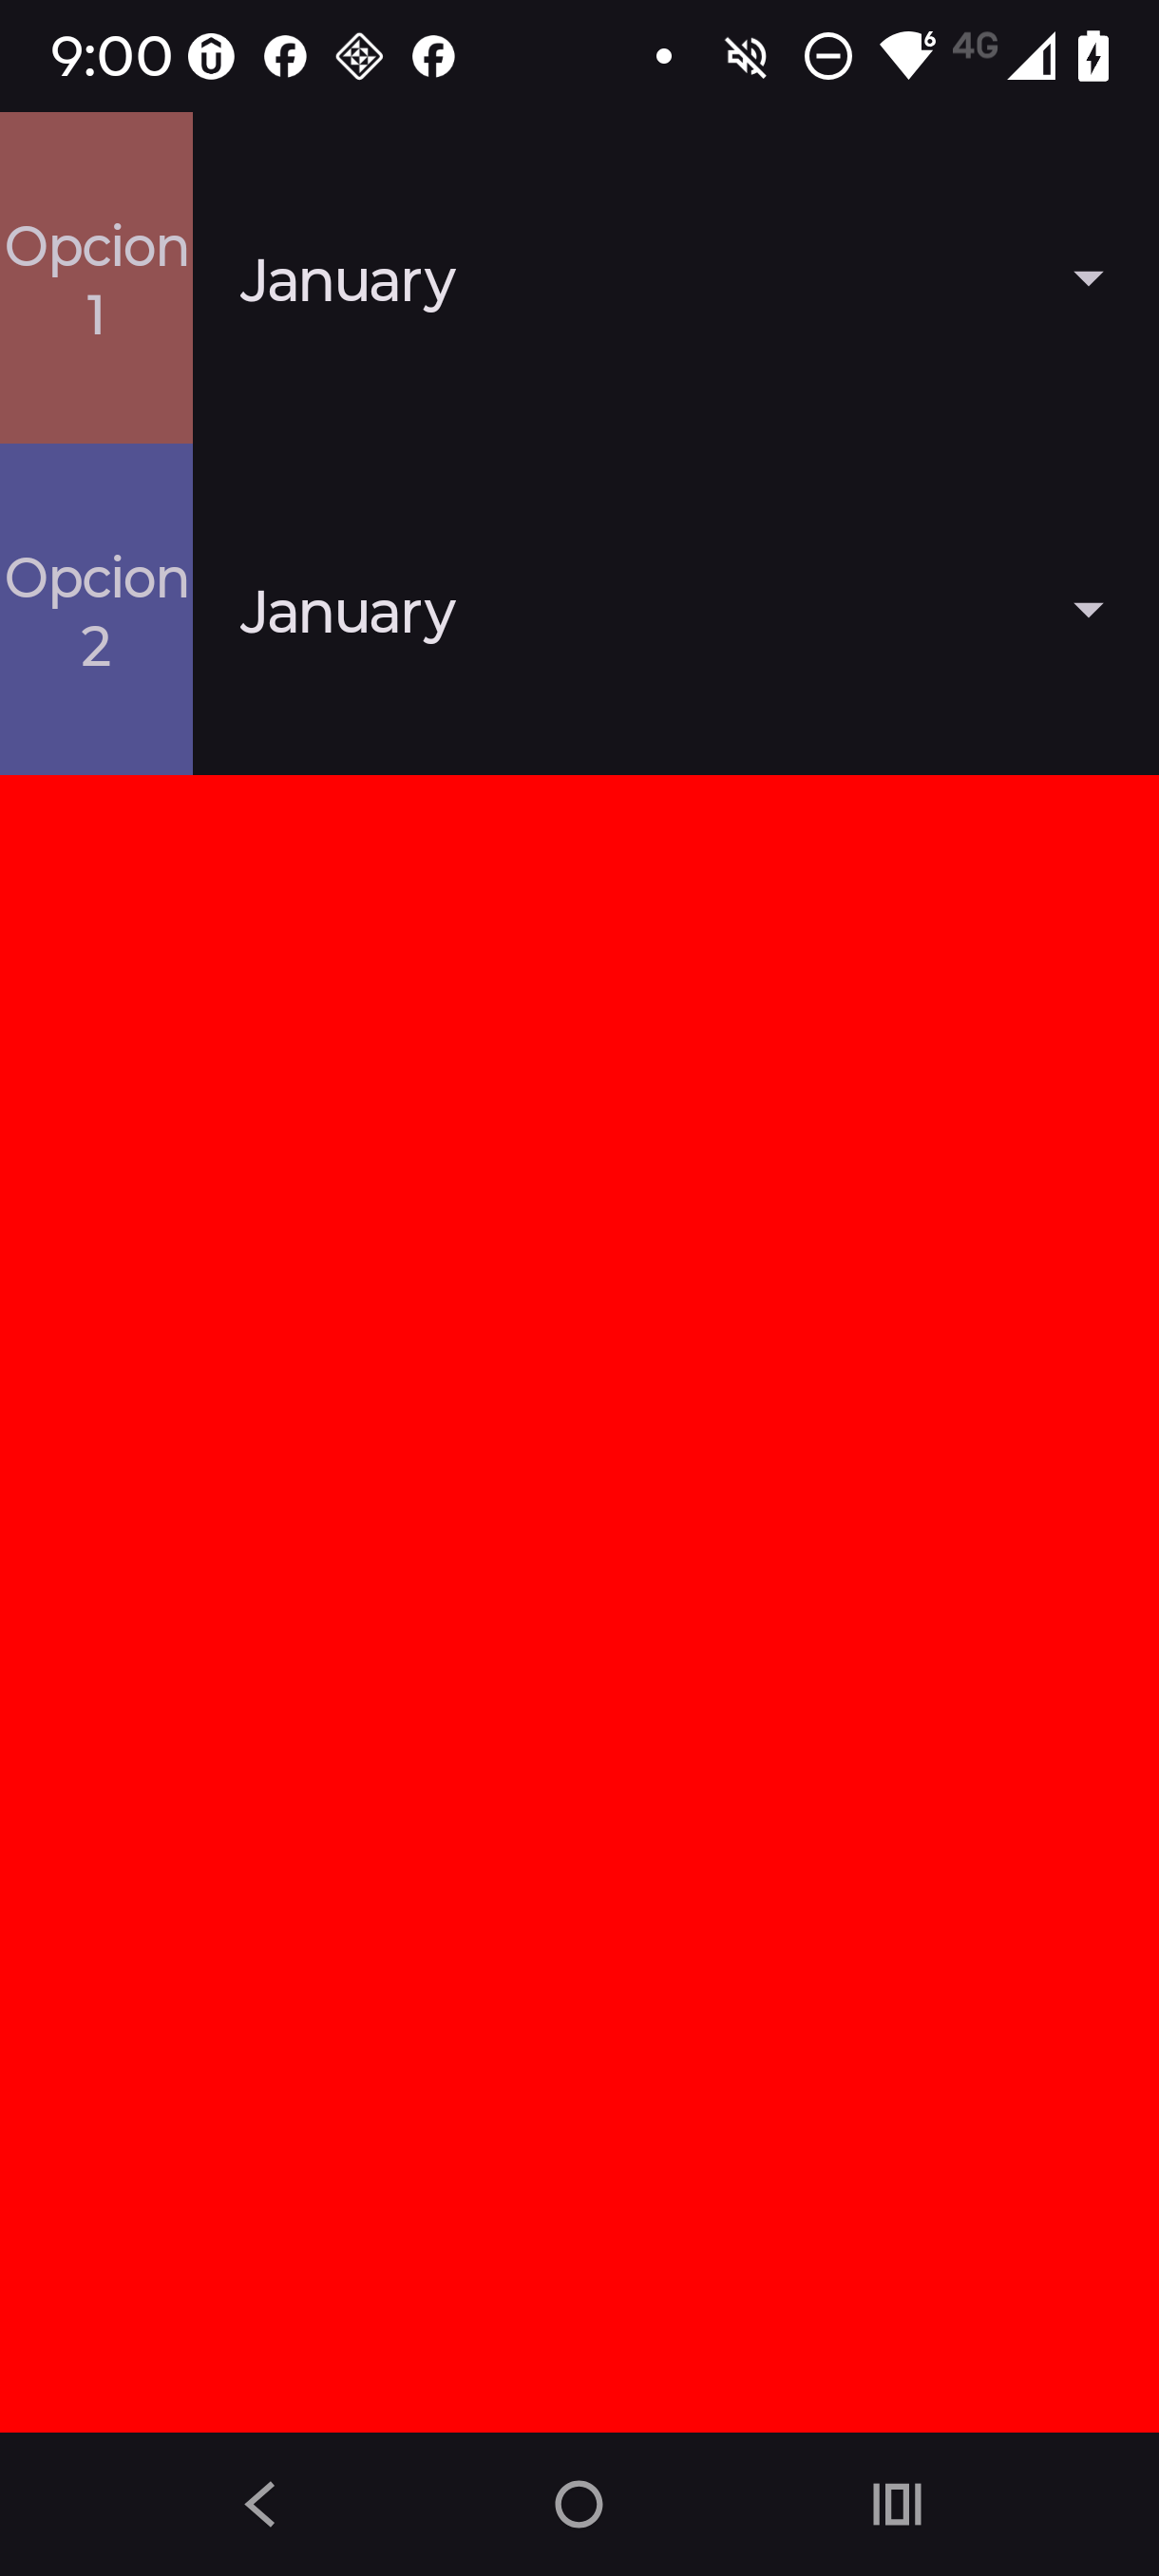
\includegraphics[width=0.98\textwidth]{02_TallerCBTis/figs/Demo07}
\end{center}

\end{columns}

\end{frame}


